%\VignetteEngine{knitr}
%\VignetteIndexEntry{prospect: a R package for processing and calibration sampling of vis-NIR spectroscopic data}
%\VignettePackage{prospect}
\documentclass[12pt]{article}\usepackage{graphicx, color}
%% maxwidth is the original width if it is less than linewidth
%% otherwise use linewidth (to make sure the graphics do not exceed the margin)
\makeatletter
\def\maxwidth{ %
  \ifdim\Gin@nat@width>\linewidth
    \linewidth
  \else
    \Gin@nat@width
  \fi
}
\makeatother

\definecolor{fgcolor}{rgb}{0.2, 0.2, 0.2}
\newcommand{\hlnumber}[1]{\textcolor[rgb]{0,0,0}{#1}}%
\newcommand{\hlfunctioncall}[1]{\textcolor[rgb]{0.501960784313725,0,0.329411764705882}{\textbf{#1}}}%
\newcommand{\hlstring}[1]{\textcolor[rgb]{0.6,0.6,1}{#1}}%
\newcommand{\hlkeyword}[1]{\textcolor[rgb]{0,0,0}{\textbf{#1}}}%
\newcommand{\hlargument}[1]{\textcolor[rgb]{0.690196078431373,0.250980392156863,0.0196078431372549}{#1}}%
\newcommand{\hlcomment}[1]{\textcolor[rgb]{0.180392156862745,0.6,0.341176470588235}{#1}}%
\newcommand{\hlroxygencomment}[1]{\textcolor[rgb]{0.43921568627451,0.47843137254902,0.701960784313725}{#1}}%
\newcommand{\hlformalargs}[1]{\textcolor[rgb]{0.690196078431373,0.250980392156863,0.0196078431372549}{#1}}%
\newcommand{\hleqformalargs}[1]{\textcolor[rgb]{0.690196078431373,0.250980392156863,0.0196078431372549}{#1}}%
\newcommand{\hlassignement}[1]{\textcolor[rgb]{0,0,0}{\textbf{#1}}}%
\newcommand{\hlpackage}[1]{\textcolor[rgb]{0.588235294117647,0.709803921568627,0.145098039215686}{#1}}%
\newcommand{\hlslot}[1]{\textit{#1}}%
\newcommand{\hlsymbol}[1]{\textcolor[rgb]{0,0,0}{#1}}%
\newcommand{\hlprompt}[1]{\textcolor[rgb]{0.2,0.2,0.2}{#1}}%

\usepackage{framed}
\makeatletter
\newenvironment{kframe}{%
 \def\at@end@of@kframe{}%
 \ifinner\ifhmode%
  \def\at@end@of@kframe{\end{minipage}}%
  \begin{minipage}{\columnwidth}%
 \fi\fi%
 \def\FrameCommand##1{\hskip\@totalleftmargin \hskip-\fboxsep
 \colorbox{shadecolor}{##1}\hskip-\fboxsep
     % There is no \\@totalrightmargin, so:
     \hskip-\linewidth \hskip-\@totalleftmargin \hskip\columnwidth}%
 \MakeFramed {\advance\hsize-\width
   \@totalleftmargin\z@ \linewidth\hsize
   \@setminipage}}%
 {\par\unskip\endMakeFramed%
 \at@end@of@kframe}
\makeatother

\definecolor{shadecolor}{rgb}{.97, .97, .97}
\definecolor{messagecolor}{rgb}{0, 0, 0}
\definecolor{warningcolor}{rgb}{1, 0, 1}
\definecolor{errorcolor}{rgb}{1, 0, 0}
\newenvironment{knitrout}{}{} % an empty environment to be redefined in TeX

\usepackage{alltt}
\usepackage[latin1]{inputenc}
\usepackage[T1]{fontenc}
\usepackage{lmodern}
\usepackage{amssymb,amsmath}
\usepackage{epstopdf} % include pdf graphics
\usepackage{graphicx} % include external graphics
\usepackage{rotating} % landscape fig and tables
\usepackage{hyperref} % for url's
\usepackage{marvosym} % for symbols
\usepackage{authblk} % manage authors and affiliations
\usepackage[cm, headings]{fullpage} % for larger margins
\usepackage{hyperref} 
\newcommand{\R}{\texttt{R} }
\newcommand{\Rfunction}[1]{{\texttt{#1}}}
\newcommand{\Robject}[1]{{\texttt{#1}}}
\newcommand{\Rargument}[1]{{\texttt{#1}}}
\newcommand{\Rpackage}[1]{{\mbox{\normalfont\textsf{#1}}}}

\hypersetup{  
  pdftitle = {An Introduction to the \Rpackage{prospect} package},
  pdfsubject = {Manuscript},
  pdfauthor = {Antoine Stevens},
  colorlinks = {true},
  linkcolor = {blue},
  citecolor = {blue},
  urlcolor = {red},
  hyperindex = {true},
  linktocpage = {true},
}

\title{An Introduction to the \Rpackage{prospect} package}
\author[1]{Antoine Stevens}
\author[2]{Leonardo Ramirez--Lopez}

\affil[1]{\footnotesize Georges Lema\^{i}tre Centre for Earth and Climate Research, Earth and Life Institute, UCLouvain, Place Pasteur 3, 1348 Louvain--La--Neuve, Belgium. \Letter~\href{mailto:antoine.stevens@uclouvain.be}{antoine.stevens@uclouvain.be}}
\affil[2]{\footnotesize Switzerland. \Letter~\href{mailto:leonardo.ramirez@wsl.ch}{leonardo.ramirez@wsl.ch}}

\date{\today}
\IfFileExists{upquote.sty}{\usepackage{upquote}}{}

\begin{document}
\maketitle

\tableofcontents

\newpage

\section{Introduction}

Visible and Near Infrared diffuse reflectance (vis--NIR) spectroscopy is a high--troughput, non--destructive and cheap sensing method that has a range of applications in agricultural, medical, food and environmental science. A number of \R packages of interest for the spectroscopist is already available for processing and analysis of spectroscopic data (Table ~\ref{tab:pck}). The CRAN task views \href{http://cran.r-project.org/web/views/Multivariate.html}{Multivariate Statistics}, \href{http://cran.r-project.org/web/views/MachineLearning.html}{Machine Learning}, \href{http://cran.r-project.org/web/views/ChemPhys.html}{Chemometrics and Computational Physics}. The interested readed can also have a look at the special issue \href{http://ww.colin-baxter.com/academic/bib/downloads/mullen07.pdf}{"Spectroscopy and Chemometrics in R"} of the Journal of Statistical Software \cite{mullen2007}.

\begin{table}[h]
\caption{Non--exhaustive list of R package useful for vis--NIR spectroscopic analysis}
\centering
\begin{tabular}{l|l}
\hline
Package Name & Description  \\
\hline
\Rpackage{chemometrics}  &  functions and scripts for chemometrics  \\
\Rpackage{ChemometricsWithR} &  functions and scripts for chemometrics       \\
\Rpackage{ChemoSpec}  &  misc functions for exploratory analysis in Spectroscopy \\
\Rpackage{hyperSpec} &  processing and visualisation of spectra   \\
\Rpackage{cluster} & cluster analysis and visualisation    \\   
\Rpackage{mvoutlier} & outlier detection in the multivariate space \\ 
\Rpackage{pls} & partial least square regression \\         
\Rpackage{signal} & signal filtering \\
\Rpackage{soil.spec} & some functions related to soil spectroscopy \\
\Rpackage{caret}  & training classification and regression models \\
\hline
\end{tabular}
\label{tab:pck}
\end{table}

The prospect package gathers algorithms commonly--used in spectroscopy for pre--treating spectra and select calibration samples. Some of the algorithms are already available in other package, like the Savitzky--Golay algorithm \cite{savitzky1964} but our functions works indifferently on \Robject{vector}, \Robject{data.frame} or \Robject{matrix} input. 

\section{Signal Processing}

The aim of signal pre--treatment is to improve data quality before modeling and remove physical information from the spectra. Applying a pre--treatment can increase the repeatability/reproducibility of the method, model robustness and accuracy, although there are no guarantees this will actually work \dots. The pre--processing functions that are currently available in the package are listed in Table ~\ref{tab:fun}.

\begin{table}[h]
\caption{List of pre--processing functions}
\centering
\begin{tabular}{l|l}
\hline
Function Name & Description  \\
\hline  \Rfunction{movav} & simple moving (or running) average filter   \\  
\Rfunction{savitzkyGolay} & Savitzky--Golay smoothing and derivative  \\      
\Rfunction{gapDer} & gap--segment derivative  \\                       
\Rfunction{continuumRemoval} & compute continuum--removed values \\                               
\Rfunction{detrend} & detrend normalization \\
\Rfunction{standardNormalVariate} & Standard Normal Variate (SNV) transformation \\
\Rfunction{binning} & average a signal in column bins \\
\Rfunction{resample} & resample a signal to new band positions \\
\Rfunction{resample2} & resample a signal using new FWHM values \\
\Rfunction{blockScale} & block scaling \\
\Rfunction{blockNorm}& sum of squares block weighting \\
\hline
\end{tabular}
\label{tab:fun}
\end{table}

We show below how they can be used, using the NIRsoil dataset included in the package \cite{fernandez2008}. Observations should be arranged row--wise.

\begin{knitrout}
\definecolor{shadecolor}{rgb}{0.969, 0.969, 0.969}\color{fgcolor}\begin{kframe}
\begin{alltt}
\hlfunctioncall{library}(prospect)
\hlfunctioncall{data}(NIRsoil)
\hlcomment{# NIRsoil is a data.frame with 825 obs and 5 variables: Nt (Total}
\hlcomment{# Nitrogen), Ciso (Carbon), CEC (Cation Exchange Capacity), train (vector}
\hlcomment{# of 0,1 indicating training (1) and validation (0) samples), spc}
\hlcomment{# (spectral matrix)}
\hlfunctioncall{str}(NIRsoil)
\end{alltt}
\begin{verbatim}
## 'data.frame':	825 obs. of  5 variables:
##  $ Nt   : num  0.3 0.69 0.71 0.85 NA ...
##  $ Ciso : num  0.22 NA NA NA 0.9 NA NA 0.6 NA 1.28 ...
##  $ CEC  : num  NA NA NA NA NA NA NA NA NA NA ...
##  $ train: num  1 1 1 1 1 1 1 1 1 1 ...
##  $ spc  : num [1:825, 1:700] 0.339 0.308 0.328 0.364 0.237 ...
##   ..- attr(*, "dimnames")=List of 2
##   .. ..$ : chr  "1" "2" "3" "4" ...
##   .. ..$ : chr  "1100" "1102" "1104" "1106" ...
\end{verbatim}
\end{kframe}
\end{knitrout}


\subsection{Noise removal}

Noise represents random fluctuations around the signal that can originate from the instrument or environmental laboratory conditions. The simplest solution to remove noise is to perform $n$ repetition of the measurements, and the average individual spectra. The noise will decrease with a factor $\sqrt{n}$. When this is not possible, or if residual noise is still present in the data, the noise can be removed mathematically. 
  
\subsubsection{Moving average or runnnig mean}

A moving average filter is a column--wise operation which average contiguous wavelengths within a given window size. 

\begin{knitrout}
\definecolor{shadecolor}{rgb}{0.969, 0.969, 0.969}\color{fgcolor}\begin{kframe}
\begin{alltt}
noisy <- NIRsoil$spc + \hlfunctioncall{rnorm}(\hlfunctioncall{length}(NIRsoil$spc), 0, 0.001)  \hlcomment{# adding some noise}
\hlcomment{# Plot the first spectrum}
\hlfunctioncall{plot}(\hlfunctioncall{as.numeric}(\hlfunctioncall{colnames}(NIRsoil$spc)), noisy[1, ], type = \hlstring{"l"}, xlab = \hlstring{"Wavelength"}, 
    ylab = \hlstring{"Absorbance"})
X <- \hlfunctioncall{movav}(noisy, w = 11)  \hlcomment{# window size of 11 bands}
\hlcomment{# Note that the 5 first and last bands are lost in the process}
\hlfunctioncall{lines}(\hlfunctioncall{as.numeric}(\hlfunctioncall{colnames}(X)), X[1, ], col = \hlstring{"red"})
\hlfunctioncall{legend}(\hlstring{"topleft"}, legend = \hlfunctioncall{c}(\hlstring{"raw"}, \hlstring{"moving average"}), lty = \hlfunctioncall{c}(1, 1), col = 1:2)
\end{alltt}
\end{kframe}\begin{figure}[]

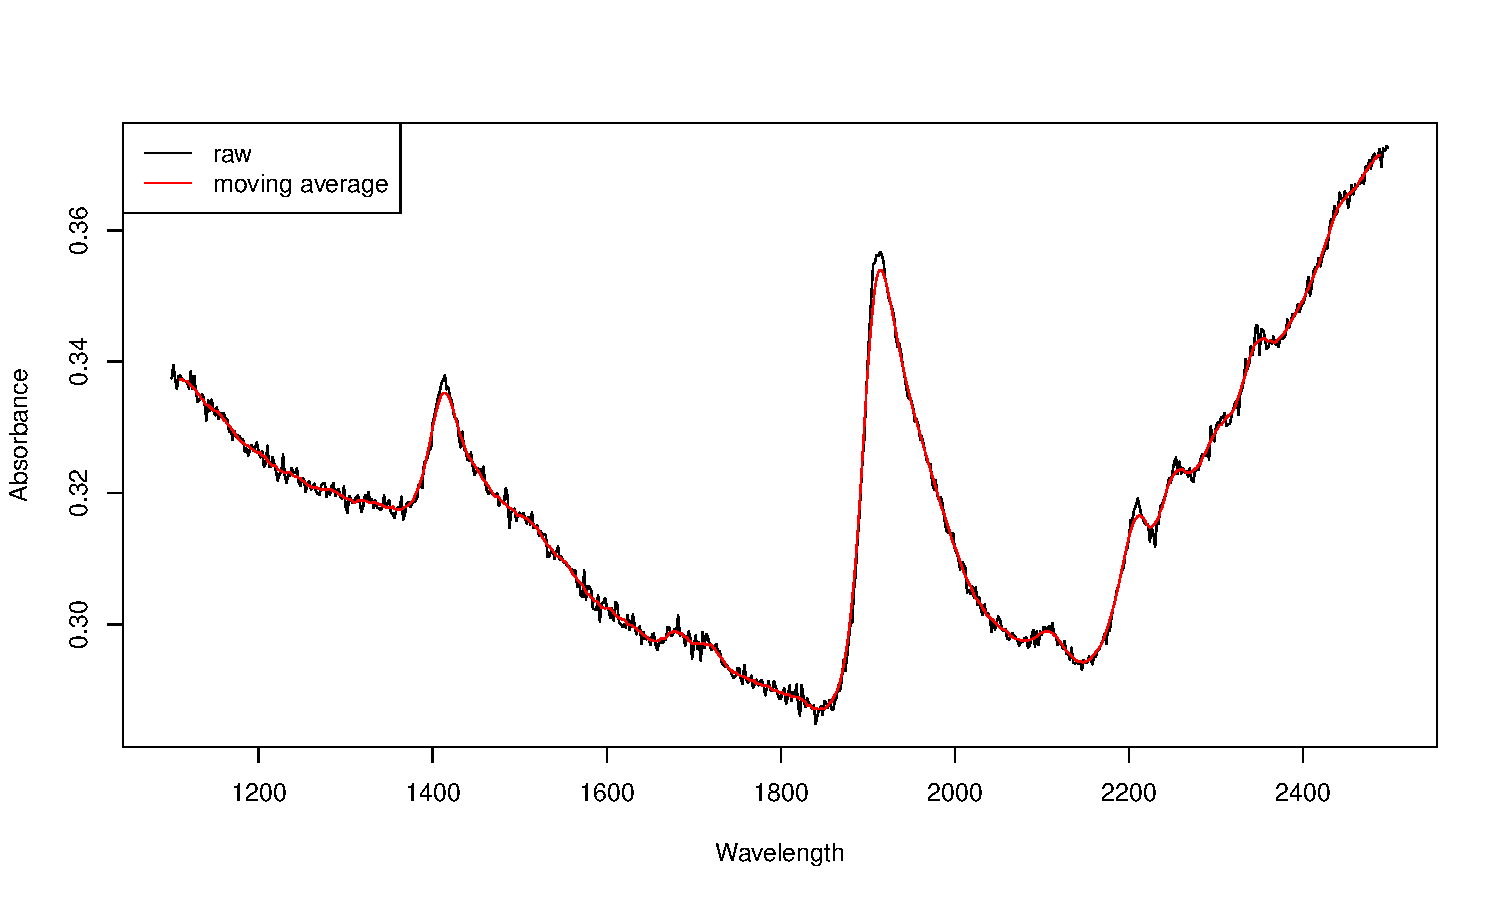
\includegraphics[width=\maxwidth]{figure/movin} \caption[Effect of a moving average with window size of 10 bands on a raw spectrum]{Effect of a moving average with window size of 10 bands on a raw spectrum\label{fig:movin}}
\end{figure}


\end{knitrout}


\subsubsection{Binning}

\begin{knitrout}
\definecolor{shadecolor}{rgb}{0.969, 0.969, 0.969}\color{fgcolor}\begin{kframe}
\begin{alltt}
\hlcomment{# After averaging, the spectrum can be further resampled (binning) We keep}
\hlcomment{# here one 1 out every 10 data points}
X.bin <- \hlfunctioncall{binning}(X, bin.size = 10)
\hlcomment{# We reduce the spectral matrix to 50 (equally-spaced) data points}
X.bin2 <- \hlfunctioncall{binning}(X, bins = 50)
\hlcomment{# Plot the first spectrum}
\hlfunctioncall{plot}(\hlfunctioncall{as.numeric}(\hlfunctioncall{colnames}(X)), X[1, ], type = \hlstring{"l"}, xlab = \hlstring{"Wavelength"}, ylab = \hlstring{"Absorbance"})
\hlcomment{# new data points}
\hlfunctioncall{points}(\hlfunctioncall{as.numeric}(\hlfunctioncall{colnames}(X.bin)), X.bin[1, ], pch = 2)
\hlfunctioncall{points}(\hlfunctioncall{as.numeric}(\hlfunctioncall{colnames}(X.bin2)), X.bin2[1, ], pch = 1, col = 2)
\hlfunctioncall{legend}(\hlstring{"topleft"}, legend = \hlfunctioncall{c}(\hlstring{"bin.size = 10"}, \hlstring{"bins = 50"}), pch = 2:1, col = 2:1)
\end{alltt}
\end{kframe}\begin{figure}[t]

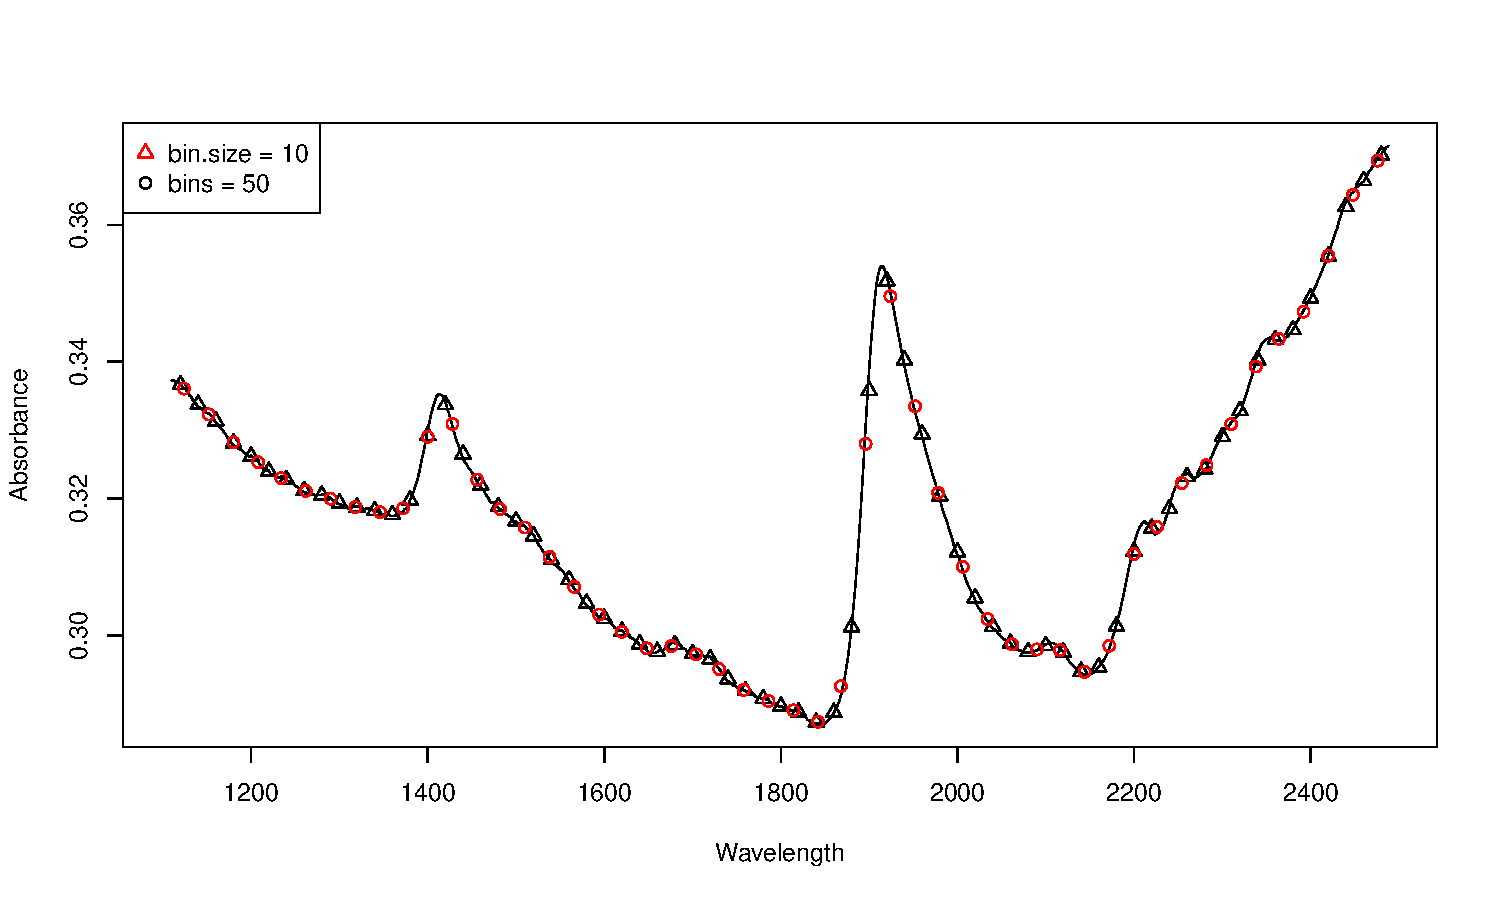
\includegraphics[width=\maxwidth]{figure/binning} \caption[Average in bins]{Average in bins\label{fig:binning}}
\end{figure}


\end{knitrout}


\subsubsection{Savitzky-Golay filtering}

Savitzky-Golay filtering \cite{savitzky1964} is a very common preprocessing technique. It fits a local polynomial regression on the signal and requires \emph{equidistant} bandwidth. Mathematically, it operates simply as a weighted sum of neighbouring values:

$$ x_j\ast = \frac{1}{N}\sum_{h=-k}^{k}{c_hx_{j+h}}$$

where $x_j\ast$ is the new value, $N$ is a normalizing coefficient, $k$ is the number of neighbour values at each side of $j$ and $c_h$ are pre--computed coefficients, that depends on the chosen polynomial order and degree (smoothing, first and second derivative)

\begin{knitrout}
\definecolor{shadecolor}{rgb}{0.969, 0.969, 0.969}\color{fgcolor}\begin{kframe}
\begin{alltt}
\hlcomment{# p = polynomial order w = window size (must be odd) m = m-th derivative}
\hlcomment{# (0 = smoothing) The function accepts vectors or matrices. For a matrix}
\hlcomment{# input, observations should be arranged row-wise}
sg.vec <- \hlfunctioncall{savitzkyGolay}(NIRsoil$spc[1, ], p = 3, w = 11, m = 0)
sg <- \hlfunctioncall{savitzkyGolay}(NIRsoil$spc, p = 3, w = 11, m = 0)
\hlcomment{# note that bands at the edges of the spectral matrix are lost !}
\hlfunctioncall{dim}(NIRsoil$spc)
\end{alltt}
\begin{verbatim}
## [1] 825 700
\end{verbatim}
\begin{alltt}
\hlfunctioncall{dim}(sg)
\end{alltt}
\begin{verbatim}
## [1] 825 690
\end{verbatim}
\end{kframe}
\end{knitrout}


\subsection{Derivatives}

Taking (numerical) derivatives of the spectra can remove both additive and multiplicative effects in the spectra and have other consequences as well (Table ~\ref{tab:der}).

\begin{table}[h]
\caption{Pro's and con's of using derivative spectra}
\centering
\begin{tabular}{l|l}
\hline
Advantage & Drawback  \\
\hline 
  Reduce of baseline offset & Risk of overfitting the calibration model \\
  Can resolve absorption overlapping & Increase noise, smoothing required \\
  Compensates for instrumental drift & Increase uncertainty in model coefficients  \\                                     
  Enhances small spectral absorptions & Complicate spectral interpretation \\
  Often increase predictive accuracy for complex datasets & Remove the baseline ! \\ 
\hline
\end{tabular}
\label{tab:der}
\end{table}

First and second derivatives of a spectrum can be computed with the finite difference method (difference between to subsequent data points), provided that the band width is constant: 

$$ x_i' = x_i - x_{i-1}$$

$$ x_i'' = x_{i-1} - 2 \cdot x_i + x_{i+1}$$

In \R, this can be simply achieved with the \Rfunction{diff} function in \Rpackage{base}: 

\begin{knitrout}
\definecolor{shadecolor}{rgb}{0.969, 0.969, 0.969}\color{fgcolor}\begin{kframe}
\begin{alltt}
\hlcomment{# X = wavelength Y = spectral matrix n = order}
d1 <- \hlfunctioncall{t}(\hlfunctioncall{diff}(\hlfunctioncall{t}(NIRsoil$spc), differences = 1))  \hlcomment{# first derivative}
d2 <- \hlfunctioncall{t}(\hlfunctioncall{diff}(\hlfunctioncall{t}(NIRsoil$spc), differences = 2))  \hlcomment{# second derivative}
\hlfunctioncall{plot}(\hlfunctioncall{as.numeric}(\hlfunctioncall{colnames}(d1)), d1[1, ], type = \hlstring{"l"}, xlab = \hlstring{"Wavelength"}, ylab = \hlstring{""})
\hlfunctioncall{lines}(\hlfunctioncall{as.numeric}(\hlfunctioncall{colnames}(d2)), d2[1, ], col = \hlstring{"red"})
\hlfunctioncall{legend}(\hlstring{"topleft"}, legend = \hlfunctioncall{c}(\hlstring{"1st der"}, \hlstring{"2nd der"}), lty = \hlfunctioncall{c}(1, 1), col = 1:2)
\end{alltt}
\end{kframe}\begin{figure}[t]

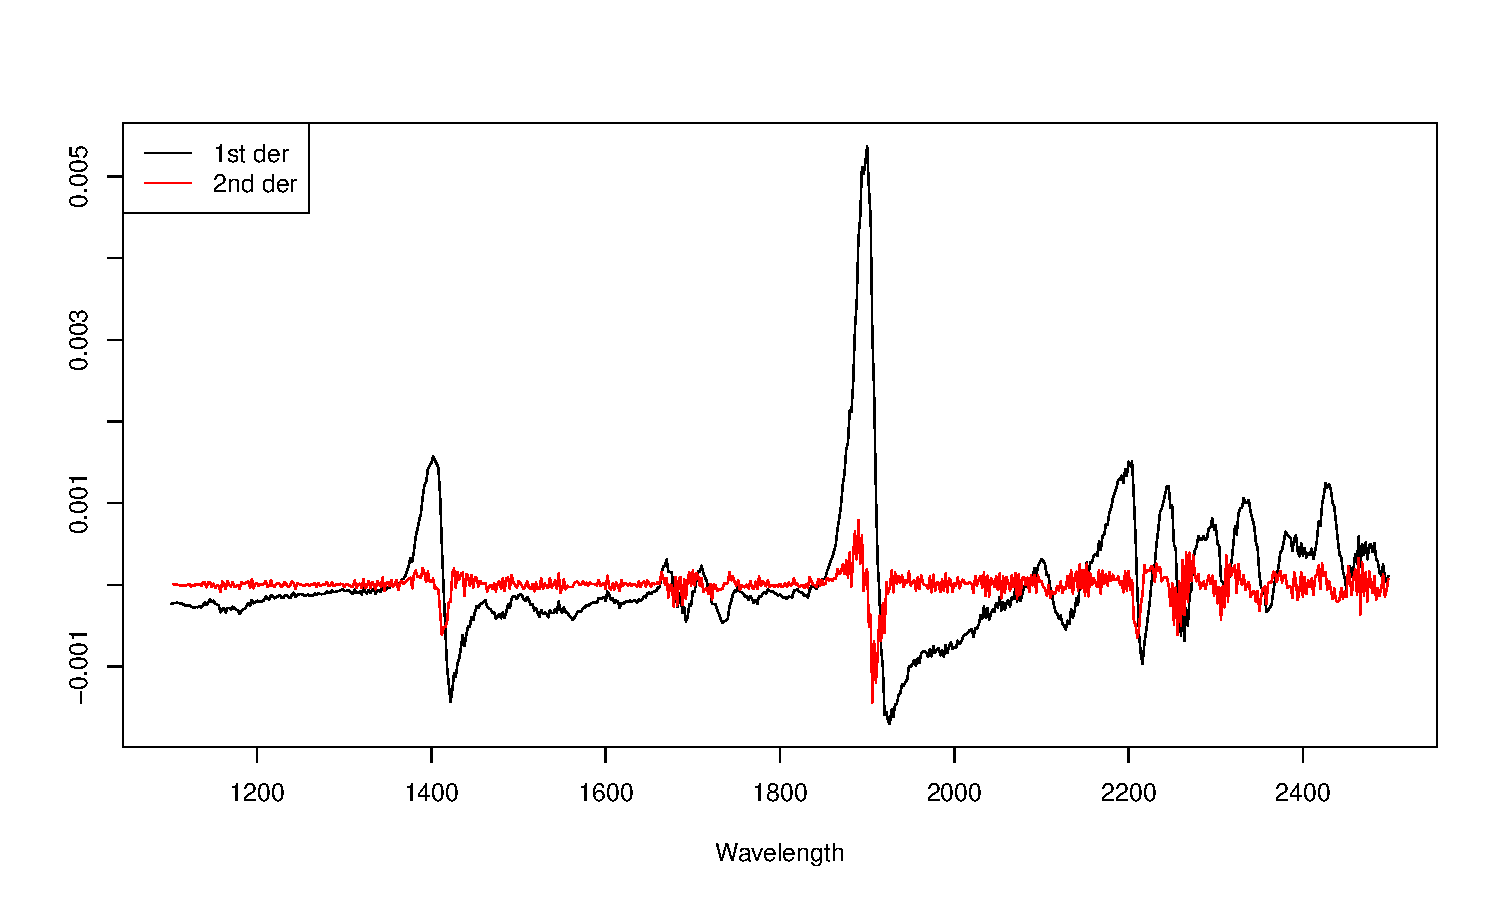
\includegraphics[width=\maxwidth]{figure/d1} \caption[Effect of first derivative and second derivative]{Effect of first derivative and second derivative\label{fig:d1}}
\end{figure}


\end{knitrout}


One can see that derivatives tend to increase noise. One can use gap derivatives or the Savitzky-Golay algorithm to solve this. The gap derivative is computed simply as:

$$ x_i' = x_{i+k} - x_{i-k}$$

$$ x_i'' = x_{i-k} - 2 \cdot x_i + x_{i+k}$$

where $k$ is the gap size. Again, this can be easily achieved in R using the \Rargument{lag} argument of the \Rfunction{diff} function

\begin{knitrout}
\definecolor{shadecolor}{rgb}{0.969, 0.969, 0.969}\color{fgcolor}\begin{kframe}
\begin{alltt}
\hlcomment{# first derivative with a gap of 10 bands}
gd1 <- \hlfunctioncall{t}(\hlfunctioncall{diff}(\hlfunctioncall{t}(NIRsoil$spc), differences = 1, lag = 10))
\end{alltt}
\end{kframe}
\end{knitrout}


For more flexibility and control over the degree of smoothing, one could however use the Savitzky-Golay (\Rfunction{savitzkyGolay}) and Gap--segment derivative (\Rfunction{gapDer}) algorithms. The Gap-segment algorithms performs first a smoothing under a given segment size, followed by gap derivative. Here is an exemple of the use of the \Rfunction{gapDer} function.


\begin{knitrout}
\definecolor{shadecolor}{rgb}{0.969, 0.969, 0.969}\color{fgcolor}\begin{kframe}
\begin{alltt}
\hlcomment{# m = order of the derivative w = window size ( = \{2 * gap size\} + 1) s =}
\hlcomment{# segment size first derivative with a gap of 10 bands}
gsd1 <- \hlfunctioncall{gapDer}(X = NIRsoil$spc, m = 1, w = 11, s = 10)
\hlfunctioncall{plot}(\hlfunctioncall{as.numeric}(\hlfunctioncall{colnames}(d1)), d1[1, ], type = \hlstring{"l"}, xlab = \hlstring{"Wavelength"}, ylab = \hlstring{""})
\hlfunctioncall{lines}(\hlfunctioncall{as.numeric}(\hlfunctioncall{colnames}(gsd1)), gsd1[1, ], col = \hlstring{"red"})
\hlfunctioncall{legend}(\hlstring{"topleft"}, legend = \hlfunctioncall{c}(\hlstring{"1st der"}, \hlstring{"gap-segment 1st der"}), lty = \hlfunctioncall{c}(1, 1), 
    col = 1:2)
\end{alltt}
\end{kframe}\begin{figure}[]

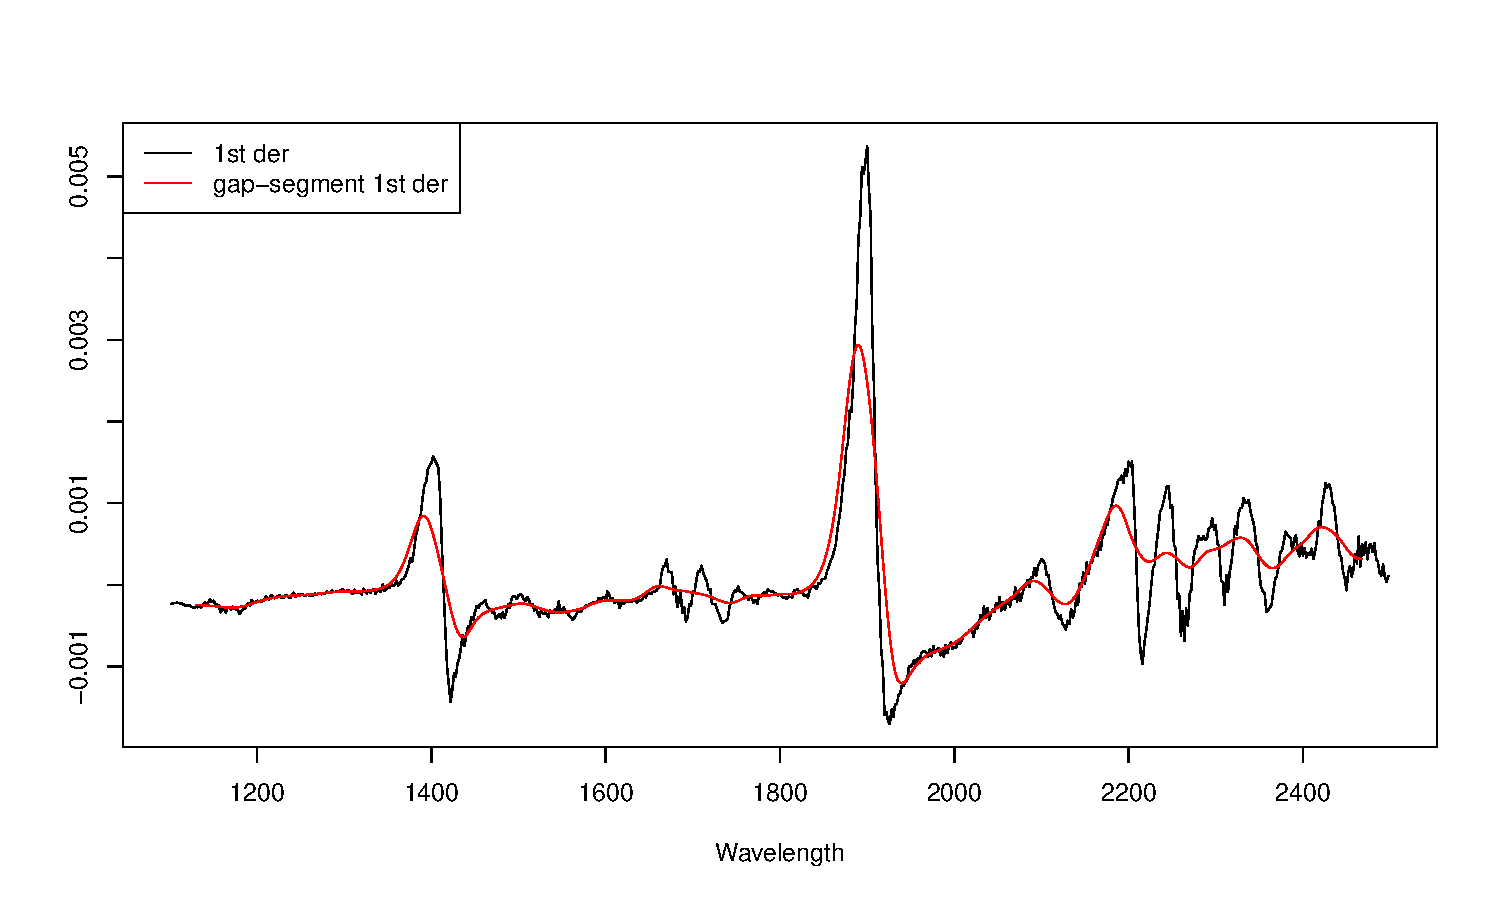
\includegraphics[width=\maxwidth]{figure/gapseg} \caption[Effect of 1st-order gap-segment derivative ]{Effect of 1st-order gap-segment derivative \label{fig:gapseg}}
\end{figure}


\end{knitrout}


\subsection{Scatter corrections}

Undesired spectral variations due to light \emph{scatter} effects and variations in effective \emph{path length} can be removed using scatter corrections.

\subsubsection{Standard Normal Variate (SNV)}

SNV is another simple way for normalizing spectra that intends to correct for light scatter. It operates row--wise:

$$ SNV_i = \frac{x_i - \bar{x_i}}{s_i}$$

\begin{knitrout}
\definecolor{shadecolor}{rgb}{0.969, 0.969, 0.969}\color{fgcolor}\begin{kframe}
\begin{alltt}
snv <- \hlfunctioncall{standardNormalVariate}(X = NIRsoil$spc)
\end{alltt}
\end{kframe}
\end{knitrout}


According to Fearn \cite{fearn2008}, it is better to perform SNV transformation after filtering (by e.g. Savitzky--Golay) than the reverse.

\subsubsection{SNV--Detrend}

The SNV--Detrend \cite{barnes1989} further accounts for wavelength-dependent scattering effects (variation in curvilinearity between the spectra). After a SNV transformation, a 2$^{nd}$--order polynomial is fit to the spectrum and subtracted from it 

\begin{knitrout}
\definecolor{shadecolor}{rgb}{0.969, 0.969, 0.969}\color{fgcolor}\begin{kframe}
\begin{alltt}
\hlcomment{# X = input spectral matrix wav = band centers}
dt <- \hlfunctioncall{detrend}(X = NIRsoil$spc, wav = \hlfunctioncall{as.numeric}(\hlfunctioncall{colnames}(NIRsoil$spc)))
\hlfunctioncall{plot}(NIRsoil$spc[1, ], type = \hlstring{"l"}, xlab = \hlstring{"Band number"}, ylab = \hlstring{""})
\hlfunctioncall{par}(new = T)
\hlfunctioncall{plot}(dt[1, ], xaxt = \hlstring{"n"}, yaxt = \hlstring{"n"}, xlab = \hlstring{""}, ylab = \hlstring{""}, col = \hlstring{"red"}, type = \hlstring{"l"})
\hlfunctioncall{axis}(4, col = \hlstring{"red"})
\hlfunctioncall{legend}(\hlstring{"topleft"}, legend = \hlfunctioncall{c}(\hlstring{"raw"}, \hlstring{"detrend signal"}), lty = \hlfunctioncall{c}(1, 1), col = 1:2)
\end{alltt}
\end{kframe}\begin{figure}[t]

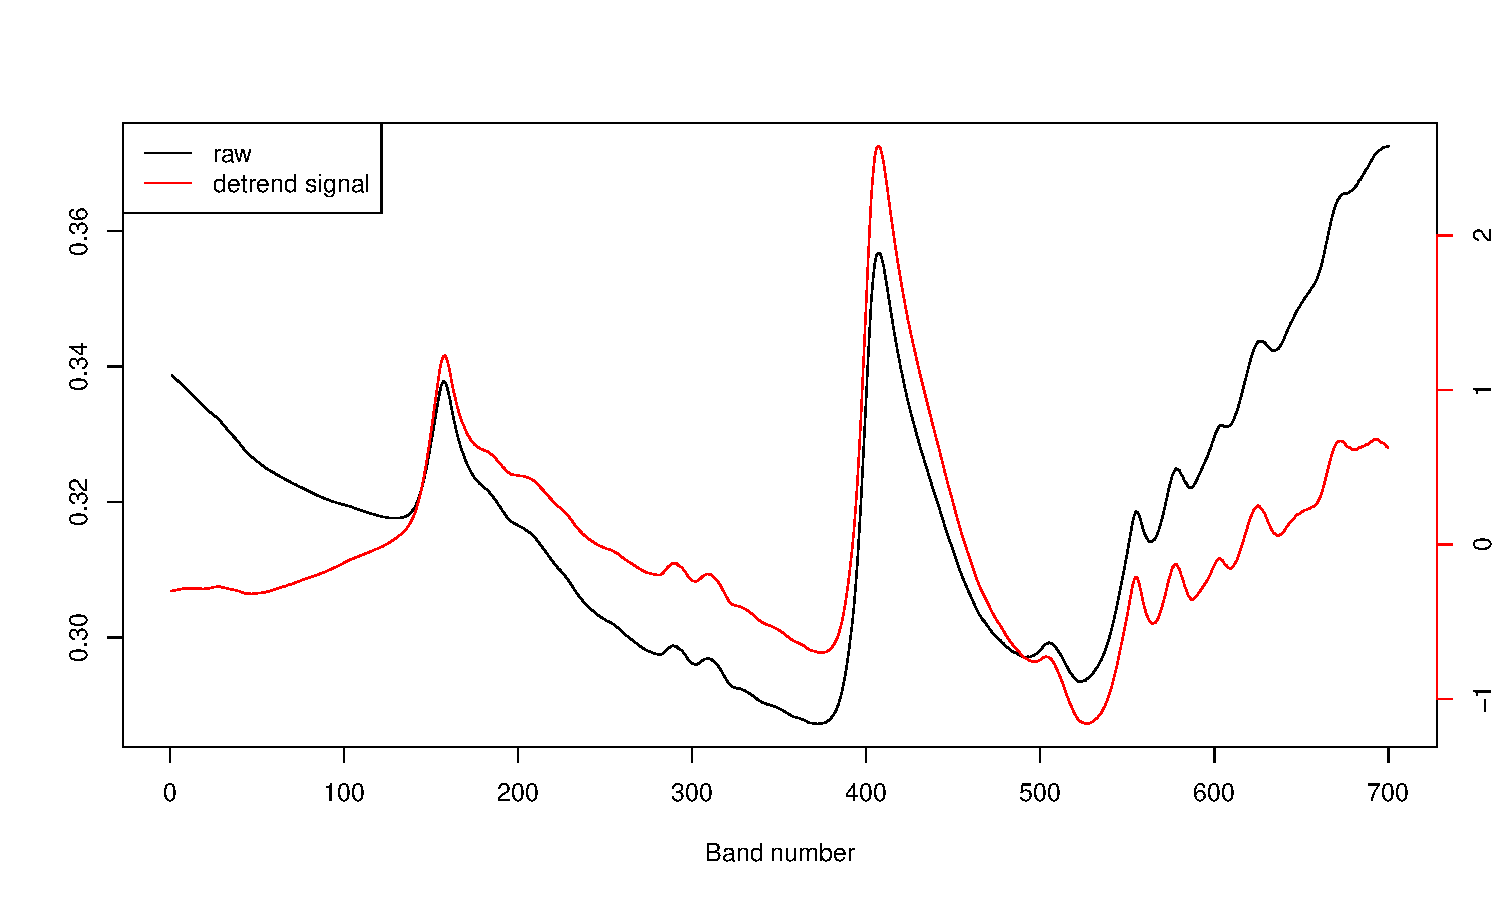
\includegraphics[width=\maxwidth]{figure/detrend} \caption[Effect of SNV-Detrend on raw spectra]{Effect of SNV-Detrend on raw spectra\label{fig:detrend}}
\end{figure}

\begin{kframe}\begin{alltt}
\hlfunctioncall{par}(new = F)
\end{alltt}
\end{kframe}
\end{knitrout}


\subsection{Centering and scaling}

Centering and scaling tranforms a given matrix to a matrix with columns with zero mean (centering), unit variance (scaling) or both (auto--scaling):

$$ Xc_{ij} = X_{ij}  - \bar{X}_{j} $$

$$ Xs_{ij} = \frac{X_{ij}  - \bar{X}_{j}}{s_{j}} $$

where $Xc$ and $Xs$ are the mean centered and auto-scaled matrices, $X$ is the input matrix, $\bar{X}_{j}$ and $s_{j}$ are the mean and standard deviation of variable $j$.

In \R, these operations are simply obtained with the \Rfunction{scale} function. Other types of scaling can be considered.  Spectroscopic models can often be improved by using ancillary data (e.g. temperature, \dots) \cite{fearn2010}. Due to the nature of spectral data (multivariate), other data would have great chance to be dominated by the spectral matrix and have no chance to contribute significantly to the model due to purely numerical reasons \cite{eriksson2006}. One can use \emph{block scaling} to overcome this limitation. It basically uses different weights for different block of variables. With \emph{soft block scaling}, each block is scaled (i.e. each column divided by a factor) such that the sum of their variance is equal to the square root of the number of variables in the block. With \emph{hard block scaling}, each block is scaled such that the sum of their variance is equal to 1.

\begin{knitrout}
\definecolor{shadecolor}{rgb}{0.969, 0.969, 0.969}\color{fgcolor}\begin{kframe}
\begin{alltt}
\hlcomment{# X = spectral matrix}
\hlcomment{# type = "soft" or "hard"}
\hlcomment{# The ouptut is a list with the scaled matrix (Xscaled) and the divisor (f)}
bs <- \hlfunctioncall{blockScale}(X=NIRsoil$spc,type=\hlstring{"hard"})$Xscaled
\hlfunctioncall{sum}(\hlfunctioncall{apply}(bs,2,var)) \hlcomment{# this works!}
\end{alltt}
\begin{verbatim}
## [1] 1
\end{verbatim}
\end{kframe}
\end{knitrout}


The problem with \emph{block scaling} is that it down--scale all the block variables to the same variance. Since sometimes this is not advised, one can alternatively use \emph{sum of squares block weighting} . The spectral matrix is multiplied by a factor to achieve a pre--determined sum of square: 

\begin{knitrout}
\definecolor{shadecolor}{rgb}{0.969, 0.969, 0.969}\color{fgcolor}\begin{kframe}
\begin{alltt}
\hlcomment{# X = spectral matrix targetnorm = desired norm for X}
bn <- \hlfunctioncall{blockNorm}(X = NIRsoil$spc, targetnorm = 1)$Xscaled
\hlfunctioncall{sum}(bn^2)  \hlcomment{# this works!}
\end{alltt}
\begin{verbatim}
## [1] 1
\end{verbatim}
\end{kframe}
\end{knitrout}


\subsection{Other transformations}

\subsubsection{Continuum removal}    

The continuum removal technique was introduced by \cite{clark1984} as an effective method to highlight absorption features of minerals. It can be viewed as an albedo normalization technique. This technique is based on the computation of the continuum (or envelope) of a given spectrum. The continuum-removed spectrum of a given spectrum is computed as follows:
\begin{enumerate}
  \item The local reflectance spectrum maxima points (in the case of absorbance, local minima points) are identified.  
  \item Then, these points are connected by linear interpolation to form the continuum $c$. 
  \item The continuum-removed spectrum is given by $\phi_{i} = \frac{x_{i}}{c_{i}};  i=\left \{ 1,..., p\right\}$, where $x_{i}$ and $c_{i}$ are the original and the continuum reflectance (or absorbance) values respectively at the $i^th$ wavelength of a set of $p$ wavelengths, and $\phi_{i}$ is the respective final reflectance (or absorbance) value after continuum removal.
\end{enumerate}

The \Rfunction{continuumRemoval} function allows to compute the continuum-removed values of either reflectance or absorbance spectra. 

\begin{knitrout}
\definecolor{shadecolor}{rgb}{0.969, 0.969, 0.969}\color{fgcolor}\begin{kframe}
\begin{alltt}
\hlcomment{# type of data: 'R' for reflectance (default), 'A' for absorbance}
cr <- \hlfunctioncall{continuumRemoval}(X = NIRsoil$spc, type = \hlstring{"A"})
\hlcomment{# plot of the 10 first abs spectra}
\hlfunctioncall{matplot}(\hlfunctioncall{as.numeric}(\hlfunctioncall{colnames}(NIRsoil$spc)), \hlfunctioncall{t}(NIRsoil$spc[1:10, ]), type = \hlstring{"l"}, 
    ylim = \hlfunctioncall{c}(0, 0.6), xlab = \hlstring{"Wavelength /nm"}, ylab = \hlstring{"Absorbance"})
\hlfunctioncall{matlines}(\hlfunctioncall{as.numeric}(\hlfunctioncall{colnames}(NIRsoil$spc)), \hlfunctioncall{t}(cr[1:10, ]))
\end{alltt}
\end{kframe}\begin{figure}[t]

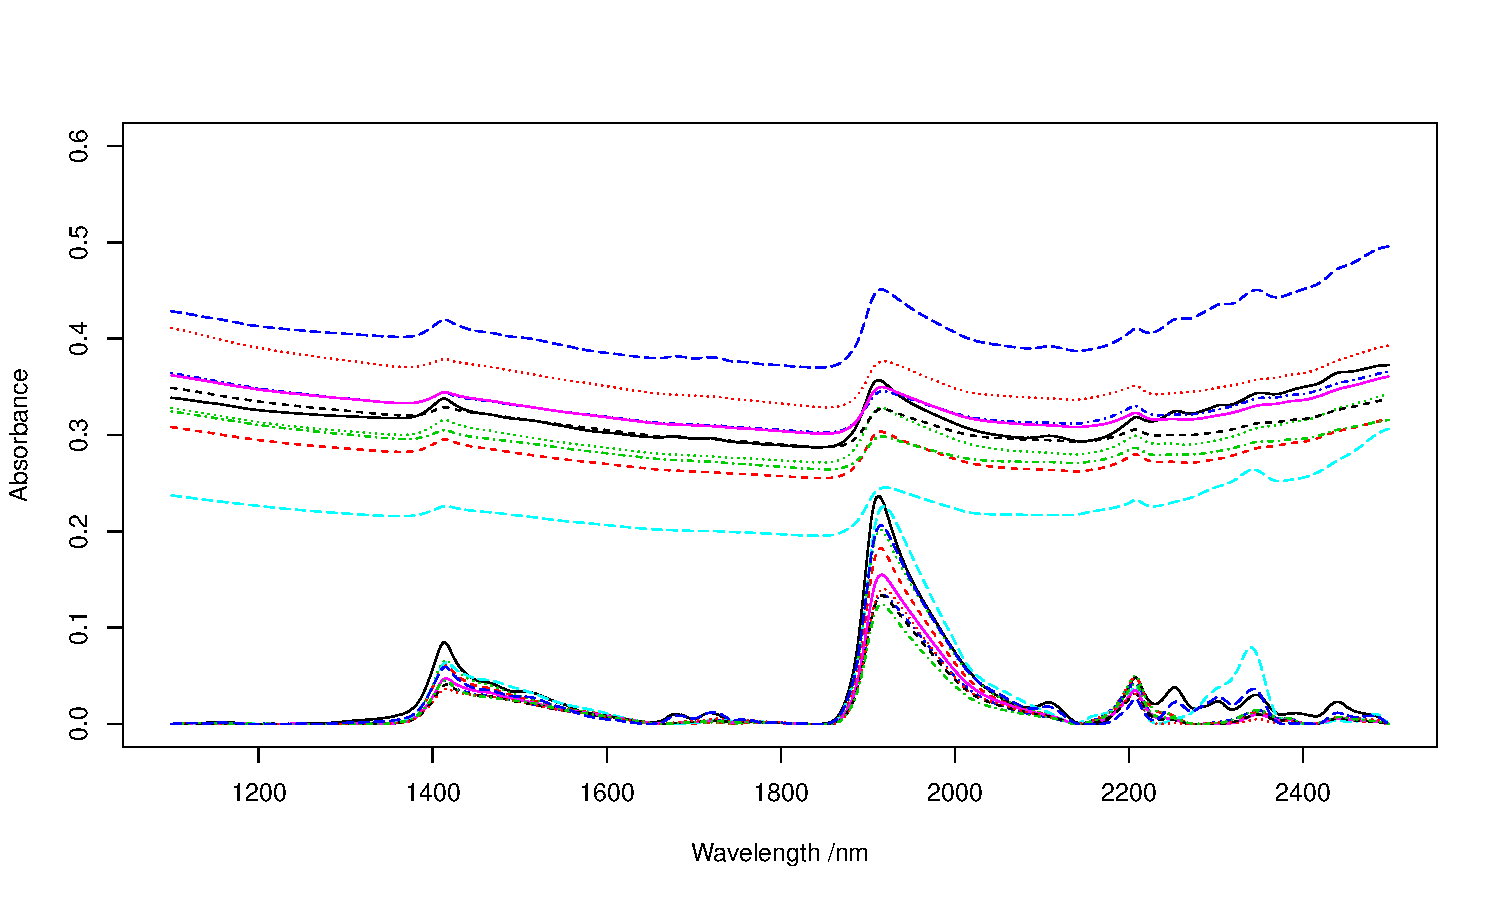
\includegraphics[width=\maxwidth]{figure/cr} \caption[Absorbance and continuum-removed absorbance spectra]{Absorbance and continuum-removed absorbance spectra\label{fig:cr}}
\end{figure}


\end{knitrout}


\subsubsection{Resampling}

To match the response of one instrument with another, a signal can be resampled to new band positions by simple interpolation (\Rfunction{resample}) or using full width half maximum (FWHM) values (\Rfunction{resample2}). 

\section{Calibration sampling algorithms }

Calibration models are usually developed on a \emph{representative} portion of the data (training set) and validated on the remaining set of samples (test/validation set). There are several solutions for selecting samples, e.g.:   
\begin{itemize}
  \item random selection (see e.g. \Rfunction{sample} function in \Rpackage{base})
  \item stratified random sampling on percentiles of the response $y$ (see e.g. \Rfunction{createDataPartion} in the \Rpackage{caret} package)
  \item  use the spectral data. 
\end{itemize}

For selecting representative samples, the \Rpackage{prospect} package provides functions that use the third solution. The following functions are available: \Rfunction{kenStone} \cite{kennard1969}, \Rfunction{duplex} \cite{snee1977}, \Rfunction{puchwein} \cite{puchwein1988}, \Rfunction{shenkWest} \cite{shenk1991}, \Rfunction{naes} \cite{naes2002}, \Rfunction{honigs} \cite{honigs1985}.

\subsection{Kennard-Stone sampling (\Rfunction{kenStone})}

To sample a subset of $n$  samples $\mathrm{X_{tr}} = \left \{ \mathrm{x_{tr}}_{j} \right \}_{j=1}^{n}$, from a given set of $N$ samples $\mathrm{X} = \left \{ \mathrm{x}_i \right \}_{i=1}^{N}$ (note that $N>n$) the Kennard-Stone sampling  algorithm consists in \cite{kennard1969}: 

\begin{enumerate}
  \item Find in $\mathrm{X}$ the samples $\mathrm{x_{tr1}}$ and  $\mathrm{x_{tr2}}$ that are the farthest apart from each other, allocate them in $\mathrm{X_{tr}}$  and remove them from $\mathrm{X}$.   
  \item Find in $\mathrm{X}$ the sample $\mathrm{x_{tr3}}$ which is the most dissimilar to the ones already allocated in $\mathrm{X_{tr}}$. Allocate $\mathrm{x_{tr3}}$ in $\mathrm{X_{tr}}$  and then remove it from $\mathrm{X}$. Note that the dissimilarity between $\mathrm{X_{tr}}$  and each $\mathrm{x}_i$  is given by the minimum distance of any sample allocated in $\mathrm{X_{tr}}$  to each $\mathrm{x}_i$. In other words, the selected sample is one of the nearest neighbours of the points already selected which is characterized by the maximum distance to the other points already selected.   
  \item Repeat the step 2 n-3 times in order to select the remaining samples ($\mathrm{x_{tr4}},..., \mathrm{x_{tr}}_n$).   

\end{enumerate}

The Kennard--Stone algorithm allows to create a calibration set that has a flat distribution over the spectral space. The metric used to compute the distance between points can be either the Euclidean distance or the Mahalanobis distance. 
Let's see some examples \dots

\begin{knitrout}
\definecolor{shadecolor}{rgb}{0.969, 0.969, 0.969}\color{fgcolor}\begin{kframe}
\begin{alltt}
\hlcomment{# Create a dataset for illustrating how the calibration sampling }
\hlcomment{# algorithms work}
X <- \hlfunctioncall{data.frame}(x1 = \hlfunctioncall{rnorm}(1000), x2 = \hlfunctioncall{rnorm}(1000))
\hlfunctioncall{plot}(X) 
\hlcomment{# kenStone produces a list with row index of the points selected for calibration}
ken <- \hlfunctioncall{kenStone}(X,k=40) 
\hlfunctioncall{points}(X[ken$model,],col=2,pch=19,cex=1.4) \hlcomment{# plot selected points}
\end{alltt}
\end{kframe}\begin{figure}[]


{\centering 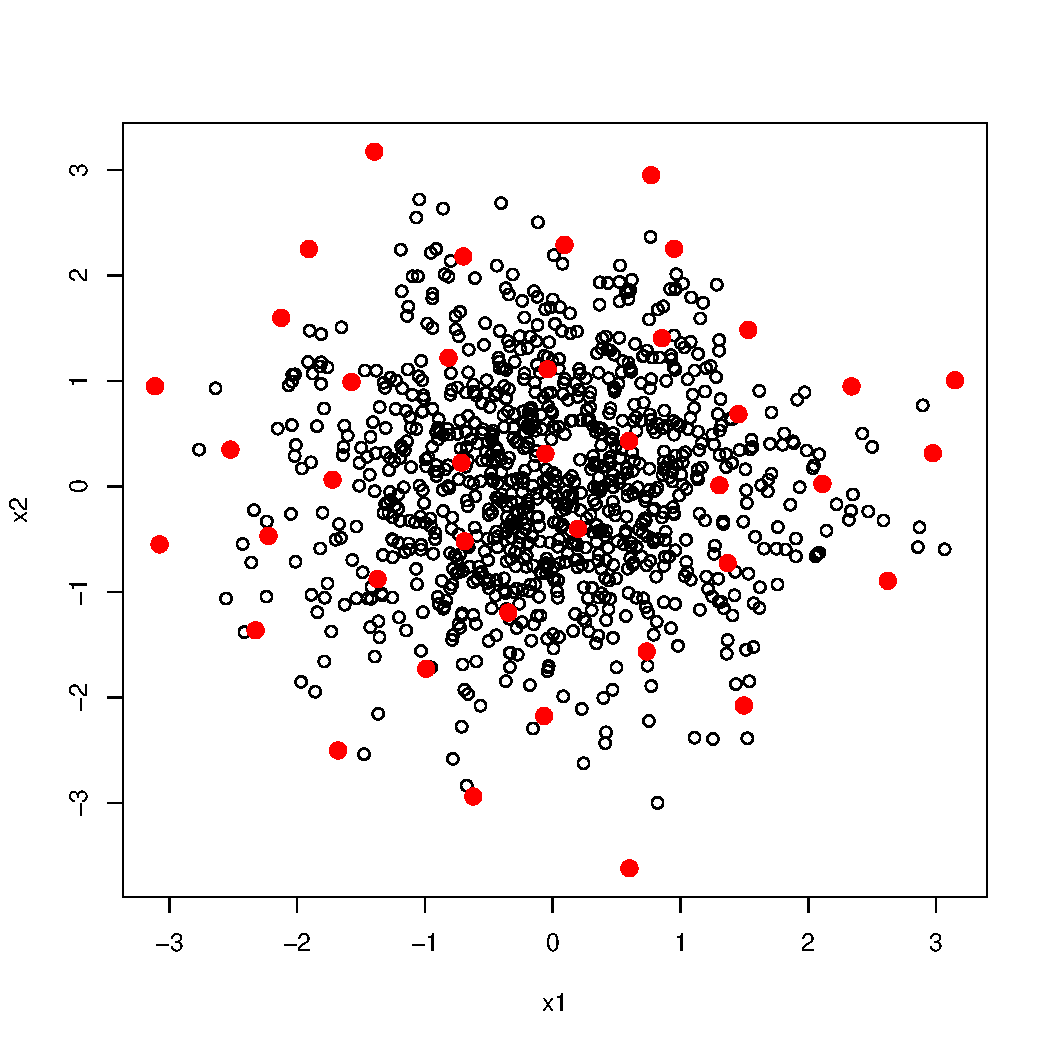
\includegraphics[width=10cm,height=10cm]{figure/ken} 

}

\caption[Selection of 40 calibration samples with the Kennard-Stone algorithm]{Selection of 40 calibration samples with the Kennard-Stone algorithm\label{fig:ken}}
\end{figure}


\end{knitrout}


\begin{knitrout}
\definecolor{shadecolor}{rgb}{0.969, 0.969, 0.969}\color{fgcolor}\begin{kframe}
\begin{alltt}

\hlcomment{# Test with the NIRsoil dataset}
\hlcomment{# one can use the mahalanobis distance}
\hlcomment{# The mahalanobis distance is computed by taking the Euclidean distance }
\hlcomment{# in the normalized principal component score space }
\hlcomment{# (see Maesschalck et al. 2000, Chemo. Int. Lab. Syst. 50, 1-18)}
\hlcomment{# If the 'pc' argument is set, the Mahalanobis distance will be used}
\hlcomment{# The 'pc' argument is the number of pc's retained in the computation of the distance}
\hlcomment{# if 'pc' < 1, then it corresponds to a treshold in terms of explained variance}
ken_mahal <- \hlfunctioncall{kenStone}(X = NIRsoil$spc, k = 20, pc= .999)
\hlcomment{# The pc components in the output list stores the pc scores}
\hlfunctioncall{plot}(ken_mahal$pc[,1],ken_mahal$pc[,2],xlab=\hlstring{"PC1"},ylab=\hlstring{"PC2"}) 
\hlcomment{# This is the selected points in the pc space}
\hlfunctioncall{points}(ken_mahal$pc[ken_mahal$model,1],ken_mahal$pc[ken_mahal$model,2],pch=19,col=2) 
\end{alltt}
\end{kframe}\begin{figure}[]


{\centering 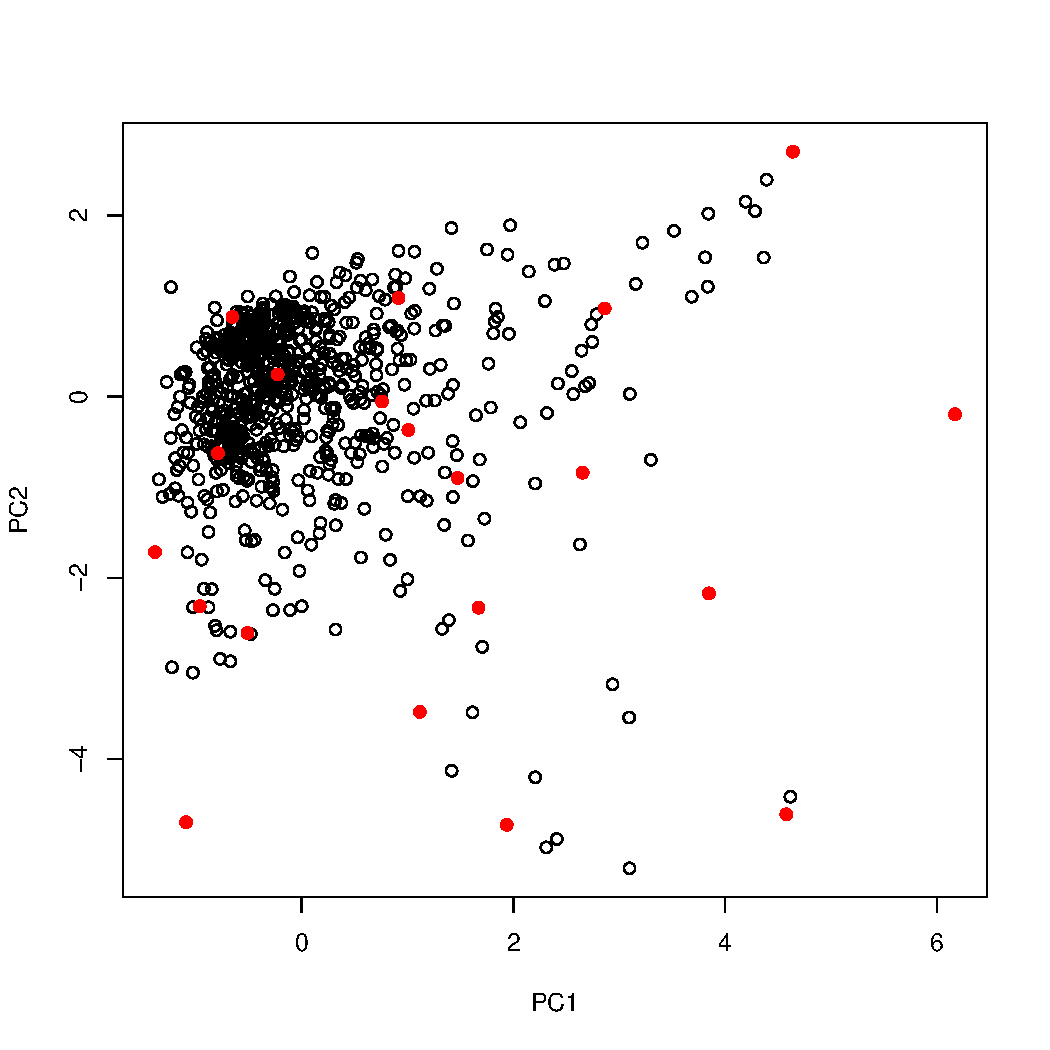
\includegraphics[width=10cm,height=10cm]{figure/ken2} 

}

\caption[Kennard-Stone sampling on the NIRsoil dataset]{Kennard-Stone sampling on the NIRsoil dataset\label{fig:ken2}}
\end{figure}


\end{knitrout}


\subsection{DUPLEX (\Rfunction{duplex})}

The Kennard--Stone algorithm selects calibration samples. Often, we need also to select a validation subset. The DUPLEX algorithm \cite{snee1977} is a modification of the Kennard-Stone which allows to select a validation set that have similar properties to the calibration set. DUPLEX, similarly to Kennard--Stone, begins by selecting pairs of points that are the farthest apart from each other, and then assigns points alternatively to the calibration and validation sets.

\begin{knitrout}
\definecolor{shadecolor}{rgb}{0.969, 0.969, 0.969}\color{fgcolor}\begin{kframe}
\begin{alltt}
dup <- \hlfunctioncall{duplex}(X = X, k = 15)  \hlcomment{# k is the number of selected samples}
\hlfunctioncall{plot}(X)
\hlfunctioncall{points}(X[dup$model, 1], X[dup$model, 2], col = \hlstring{"red"}, pch = 19)  # calibration samples
\hlfunctioncall{points}(X[dup$test, 1], X[dup$test, 2], col = \hlstring{"blue"}, pch = 17)  # validation samples
\hlfunctioncall{legend}(\hlstring{"topright"}, legend = \hlfunctioncall{c}(\hlstring{"calibration"}, \hlstring{"validation"}), pch = \hlfunctioncall{c}(19, 17), 
    col = \hlfunctioncall{c}(\hlstring{"red"}, \hlstring{"blue"}))
\end{alltt}
\end{kframe}\begin{figure}[]


{\centering 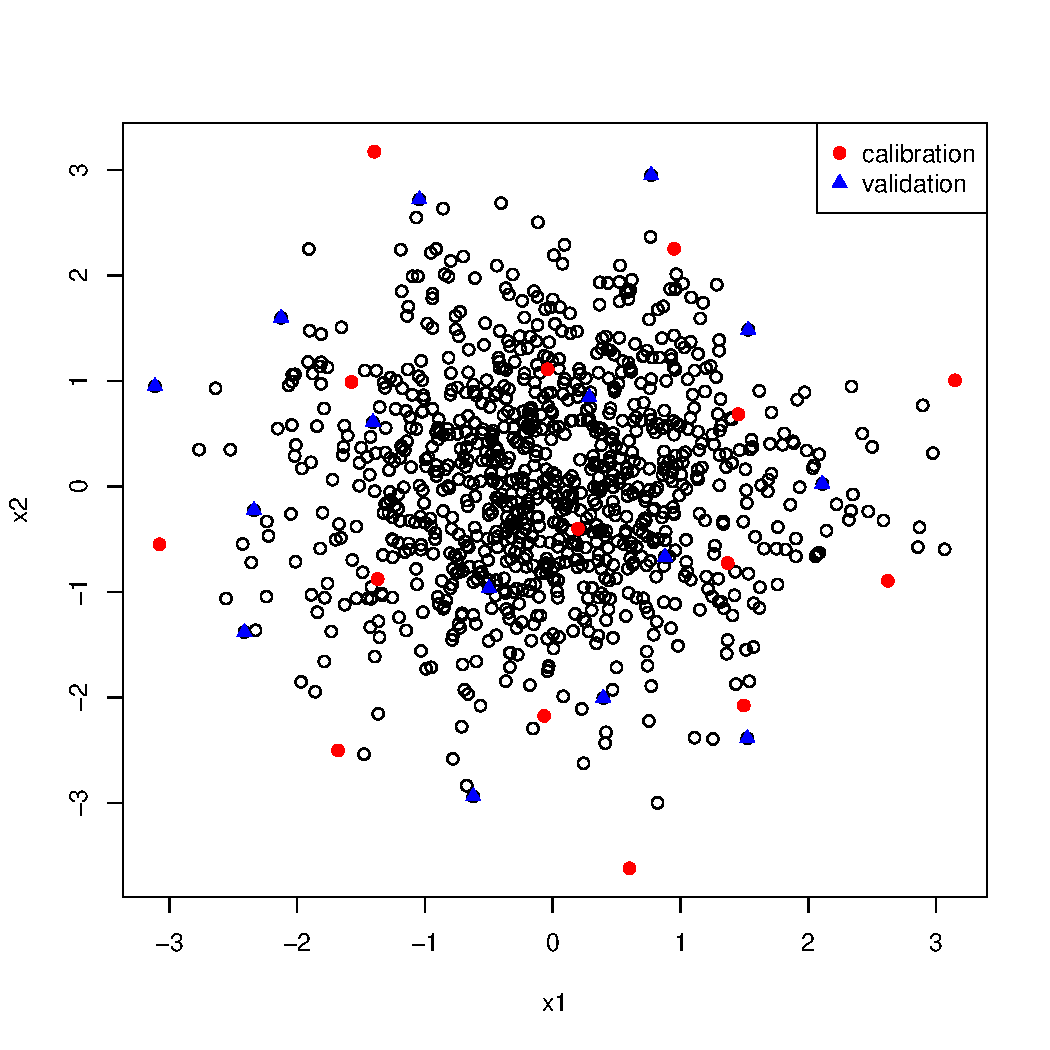
\includegraphics[width=10cm,height=10cm]{figure/duplex} 

}

\caption[Selection of 15 calibration and validation samples with the DUPLEX algorithm]{Selection of 15 calibration and validation samples with the DUPLEX algorithm\label{fig:duplex}}
\end{figure}


\end{knitrout}


\subsection{$k$-means sampling (\Rfunction{naes})}

The $k$-means sampling simply uses $k$-means clustering algorithm. To sample a subset of $n$  samples $\mathrm{X_{tr}} = \left \{ \mathrm{x_{tr}}_{j} \right \}_{j=1}^{n}$, from a given set of $N$ samples $\mathrm{X} = \left \{ \mathrm{x}_i \right \}_{i=1}^{N}$ (note that $N>n$) the algorithm works as follows:  

\begin{enumerate}
  \item Perform a $k$-means clustering of $\mathrm{X}$ using $n$ clusters.   
  \item Extract the $n$ centroids ($c$, or prototypes). This can be also the sample that is the farthest away from the centre of the data, or a random selection. See the \Rargument{method} argument in \Rfunction{naes}.
  \item Calculate the distance of each sample to each $c$.  
  \item For each $c$ allocate in $\mathrm{X_{tr}}$ its closest sample found in $\mathrm{X}$.  
\end{enumerate}

\begin{knitrout}
\definecolor{shadecolor}{rgb}{0.969, 0.969, 0.969}\color{fgcolor}\begin{kframe}
\begin{alltt}
\hlcomment{# X = the input matrix}
\hlcomment{# k = number of calibration samples to be selected}
\hlcomment{# pc = if pc is specified, k-mean is performed in the pc space }
\hlcomment{# (here we will use only the two 1st pcs)}
\hlcomment{# iter.max =  maximum number of iterations allowed for the k-means clustering.}
kms <- \hlfunctioncall{naes}(X = NIRsoil$spc, k = 5, pc = 2, iter.max = 100)
\hlcomment{# Plot the pcs scores and clusters}
\hlfunctioncall{plot}(kms$pc,col=kms$cluster) 
\hlcomment{# Add the selected points}
\hlfunctioncall{points}(kms$pc[kms$model,],col=6,pch=19)
\end{alltt}
\end{kframe}\begin{figure}[]


{\centering 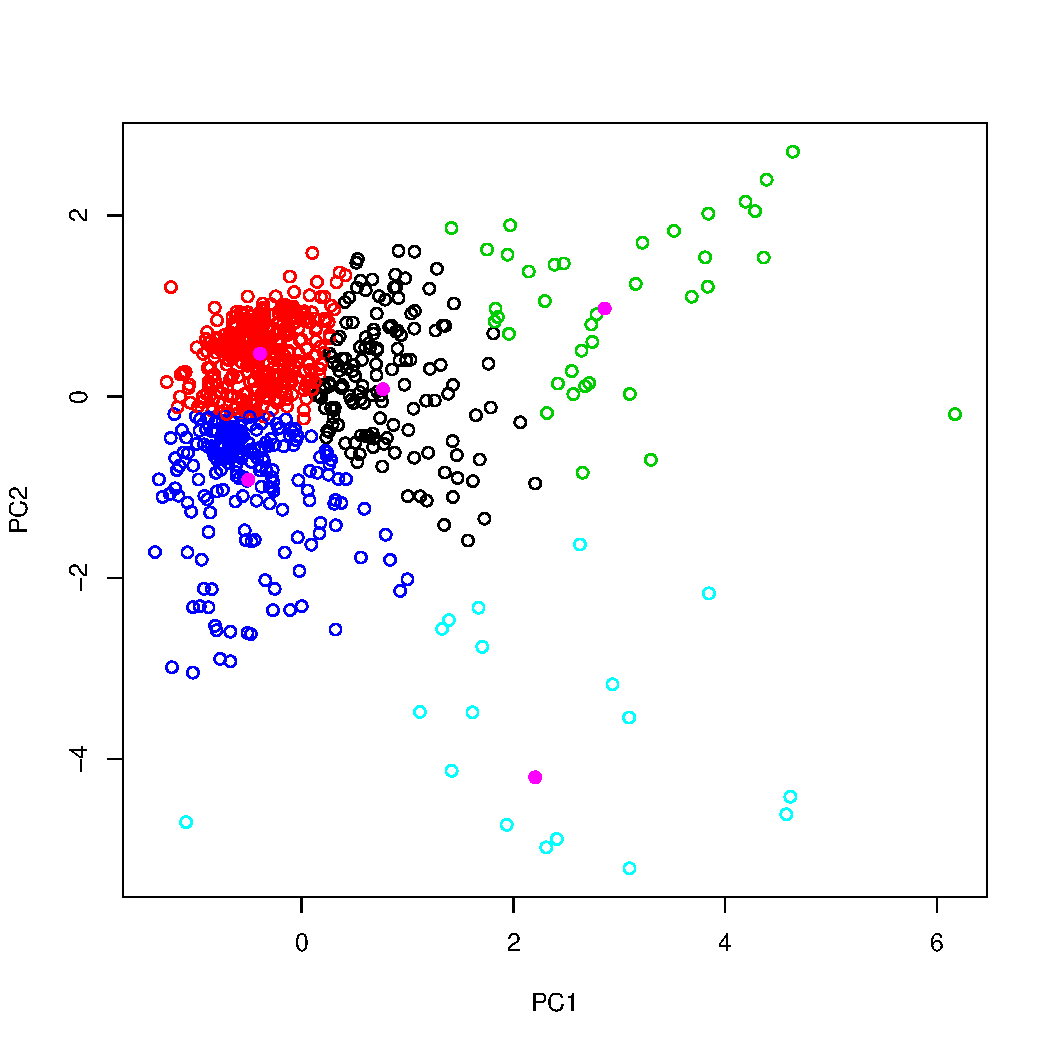
\includegraphics[width=10cm,height=10cm]{figure/naes} 

}

\caption[Selection of 5 samples by k-means sampling]{Selection of 5 samples by k-means sampling\label{fig:naes}}
\end{figure}


\end{knitrout}


\subsection{SELECT algorithm (\Rfunction{shenkWest})}

The SELECT algorithm \cite{shenk1991} is an iterative procedure which selects the sample having the maximum number of neighbour samples within a given distance (\Rargument{d.min} argument) and remove the neighbour samples of the selected sample from the list of points. The number of selected samples depends on the chosen treshold (default = 0.6). The distance metric is the Mahalanobis distance divided by the number of dimensions (number of pc components) used to compute the distance. Here is an example of how the \Rfunction{shenkWest} function might work:

\begin{knitrout}
\definecolor{shadecolor}{rgb}{0.969, 0.969, 0.969}\color{fgcolor}\begin{kframe}
\begin{alltt}
shenk <- \hlfunctioncall{shenkWest}(X = NIRsoil$spc, d.min = 0.6, pc = 2)
\hlfunctioncall{plot}(shenk$pc)
\hlfunctioncall{points}(shenk$pc[shenk$model, ], col = 2, pch = 19)
\end{alltt}
\end{kframe}\begin{figure}[]


{\centering 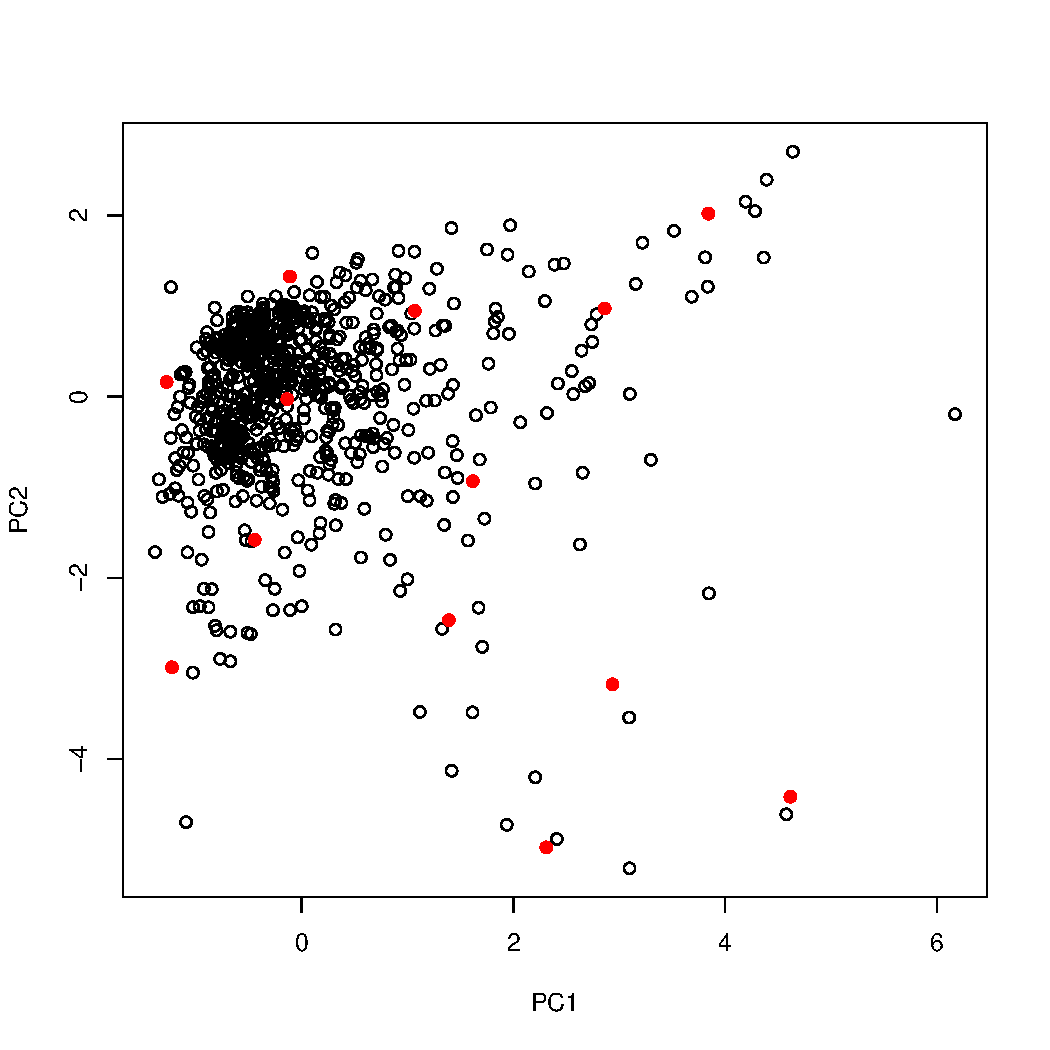
\includegraphics[width=10cm,height=10cm]{figure/shenk} 

}

\caption[Selection of samples with the SELECT algorithm]{Selection of samples with the SELECT algorithm\label{fig:shenk}}
\end{figure}


\end{knitrout}


\subsection{Puchwein algorithm (\Rfunction{puchwein})}

The Puchwein algorithm is yet another algorithm for calibration sampling \cite{puchwein1988} that creates a calibration set with a flat distribution. A nice feature of the algorithm is that it allows an objective selection of the number of required calibration samples with the help of plots. First the data is usually reduced through PCA and the most significant PCs are retained. Then the mahalanobis distance ($H$) to the center of the matrix is computed and samples are sorted decreasingly. The distances betwwen samples in the PC space are then computed.

Here is a \emph{pseudo-code} of the algorithm:

\begin{quote}
\begin{enumerate}
  \item Definition of a limiting distance
  \item Find the sample with $\max(H)$
  \item Remove all the samples which are within the limiting distance away from the sample selected in step 2.
  \item Go back in step 2 and find the sample with $\max(H)$ within the remaining samples
  \item When there is no sample anymore, go back to step 1 and increase the limiting distance.
\end{enumerate}
\end{quote}

\begin{knitrout}
\definecolor{shadecolor}{rgb}{0.969, 0.969, 0.969}\color{fgcolor}\begin{kframe}
\begin{alltt}
pu <- \hlfunctioncall{puchwein}(X = NIRsoil$spc, k = 0.2, pc = 2)
\hlfunctioncall{plot}(pu$pc)
\hlfunctioncall{points}(pu$pc[pu$model, ], col = 2, pch = 19)  \hlcomment{# selected samples}
\end{alltt}
\end{kframe}\begin{figure}[]


{\centering 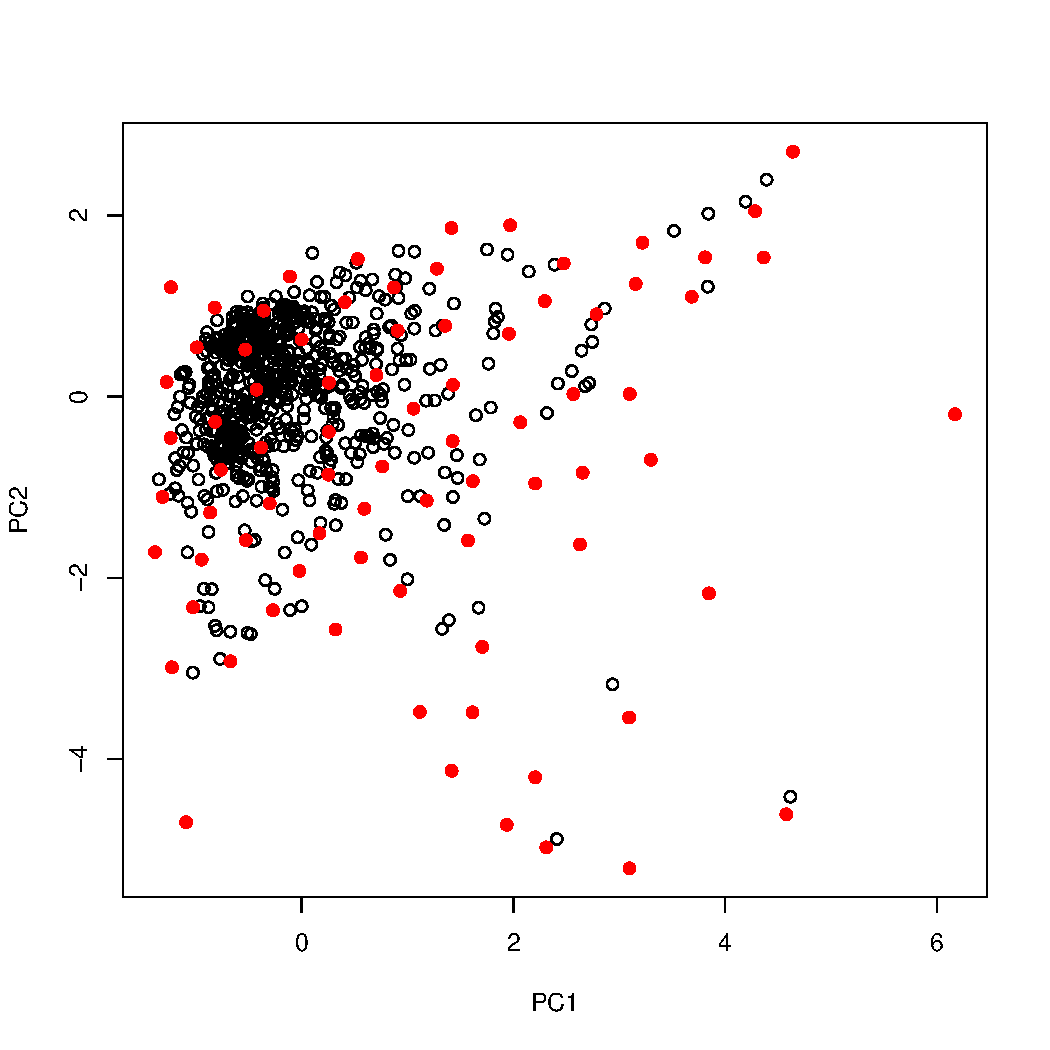
\includegraphics[width=10cm,height=10cm]{figure/puchwein} 

}

\caption[Samples selected by the Puchwein algorithm]{Samples selected by the Puchwein algorithm\label{fig:puchwein}}
\end{figure}


\end{knitrout}


The number of sample selected depends on the limiting distance. To help choosing the appropriate number of samples, two plots are used \cite{shetty2012}:
\begin{itemize}
  \item a plot showing the number of samples that are removed in each loop and the total number of samples left
  \item a plot showing the theoretical sum of leverages (each sample has the same leverage) together with the true sum of leverages. The number of samples removed that reach the maximum difference between the two can be considered to be optimal
\end{itemize}


\begin{knitrout}
\definecolor{shadecolor}{rgb}{0.969, 0.969, 0.969}\color{fgcolor}\begin{kframe}
\begin{alltt}
\hlcomment{# Optimal loop}
\hlfunctioncall{par}(mfrow = \hlfunctioncall{c}(2, 1))
\hlfunctioncall{plot}(pu$leverage$removed, pu$leverage$diff, type = \hlstring{"l"}, xlab = \hlstring{"# samples removed"}, 
    ylab = \hlstring{"Difference between th. and obs sum of leverages"})
\hlfunctioncall{plot}(pu$leverage$loop, \hlfunctioncall{nrow}(NIRsoil) - pu$leverage$removed, xlab = \hlstring{"# loops"}, 
    ylab = \hlstring{"# samples kept"}, type = \hlstring{"l"})
\end{alltt}
\end{kframe}\begin{figure}[]

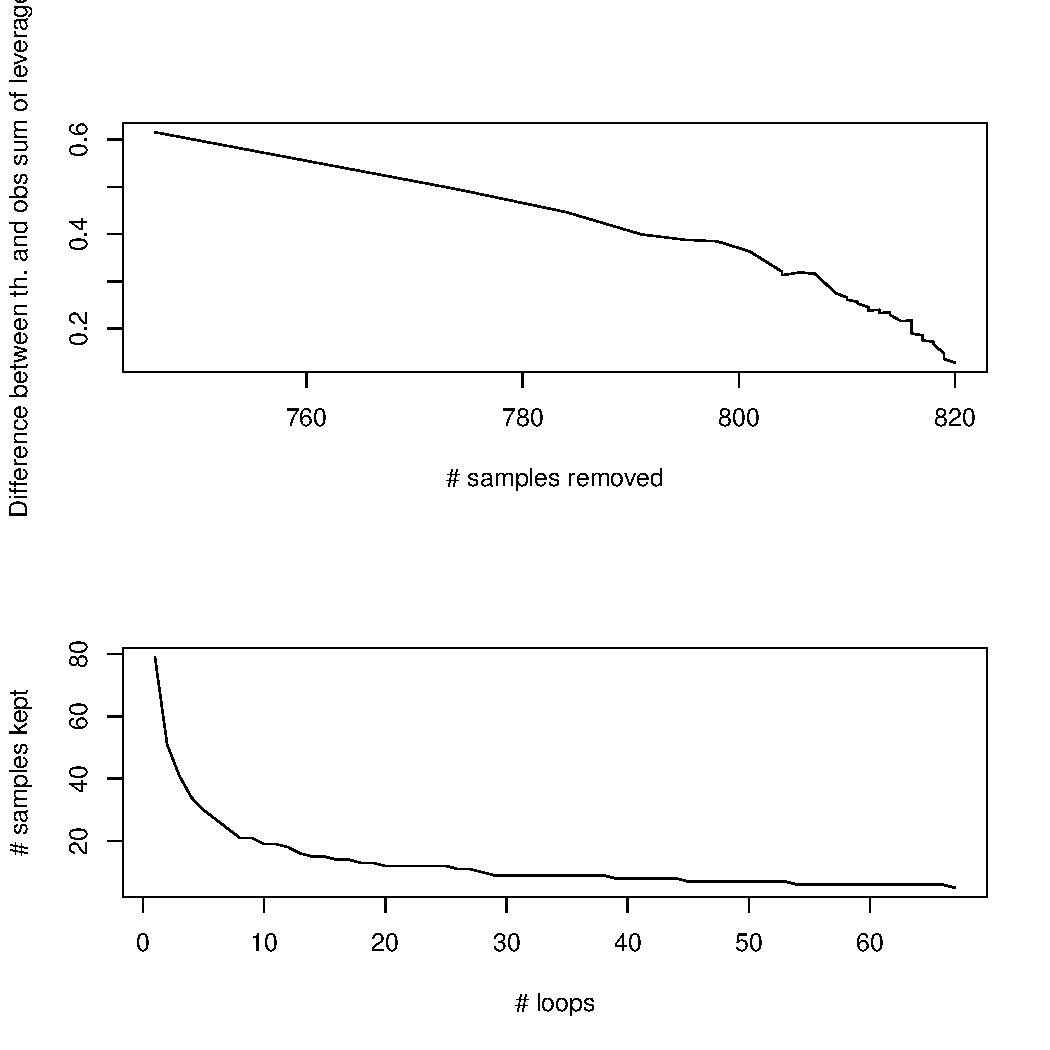
\includegraphics[width=\maxwidth]{figure/puchwein2} \caption[How to find the optimal loop]{How to find the optimal loop\label{fig:puchwein2}}
\end{figure}

\begin{kframe}\begin{alltt}
\hlfunctioncall{par}(mfrow = \hlfunctioncall{c}(1, 1))
\hlcomment{# This basically shows that the first loop is optimal}
\end{alltt}
\end{kframe}
\end{knitrout}


\subsection{Honigs (\Rfunction{honigs})}

The Honigs algorithm selects samples based on the size of their absorption features \cite{honigs1985}. It can works both on absorbance and continuum-removed spectra. The sample having the highest absorption feature is selected first. Then this absorption is substracted from other spectra and the algorithm iteratively select samples with the highest absorption (in absolute value) until the desired number of samples is reached.


\begin{knitrout}
\definecolor{shadecolor}{rgb}{0.969, 0.969, 0.969}\color{fgcolor}\begin{kframe}
\begin{alltt}
ho <- \hlfunctioncall{honigs}(X = NIRsoil$spc, k = 10, type = \hlstring{"A"})
\hlcomment{# plot calibration spectra}
\hlfunctioncall{matplot}(\hlfunctioncall{as.numeric}(\hlfunctioncall{colnames}(NIRsoil$spc)), \hlfunctioncall{t}(NIRsoil$spc[ho$model, ]), type = \hlstring{"l"}, 
    xlab = \hlstring{"Wavelength"}, ylab = \hlstring{"Absorbance"})
\hlcomment{# add bands used during the selection process}
\hlfunctioncall{abline}(v = \hlfunctioncall{as.numeric}(\hlfunctioncall{colnames}(NIRsoil$spc))[ho$bands], lty = 2)
\end{alltt}
\end{kframe}\begin{figure}[h]

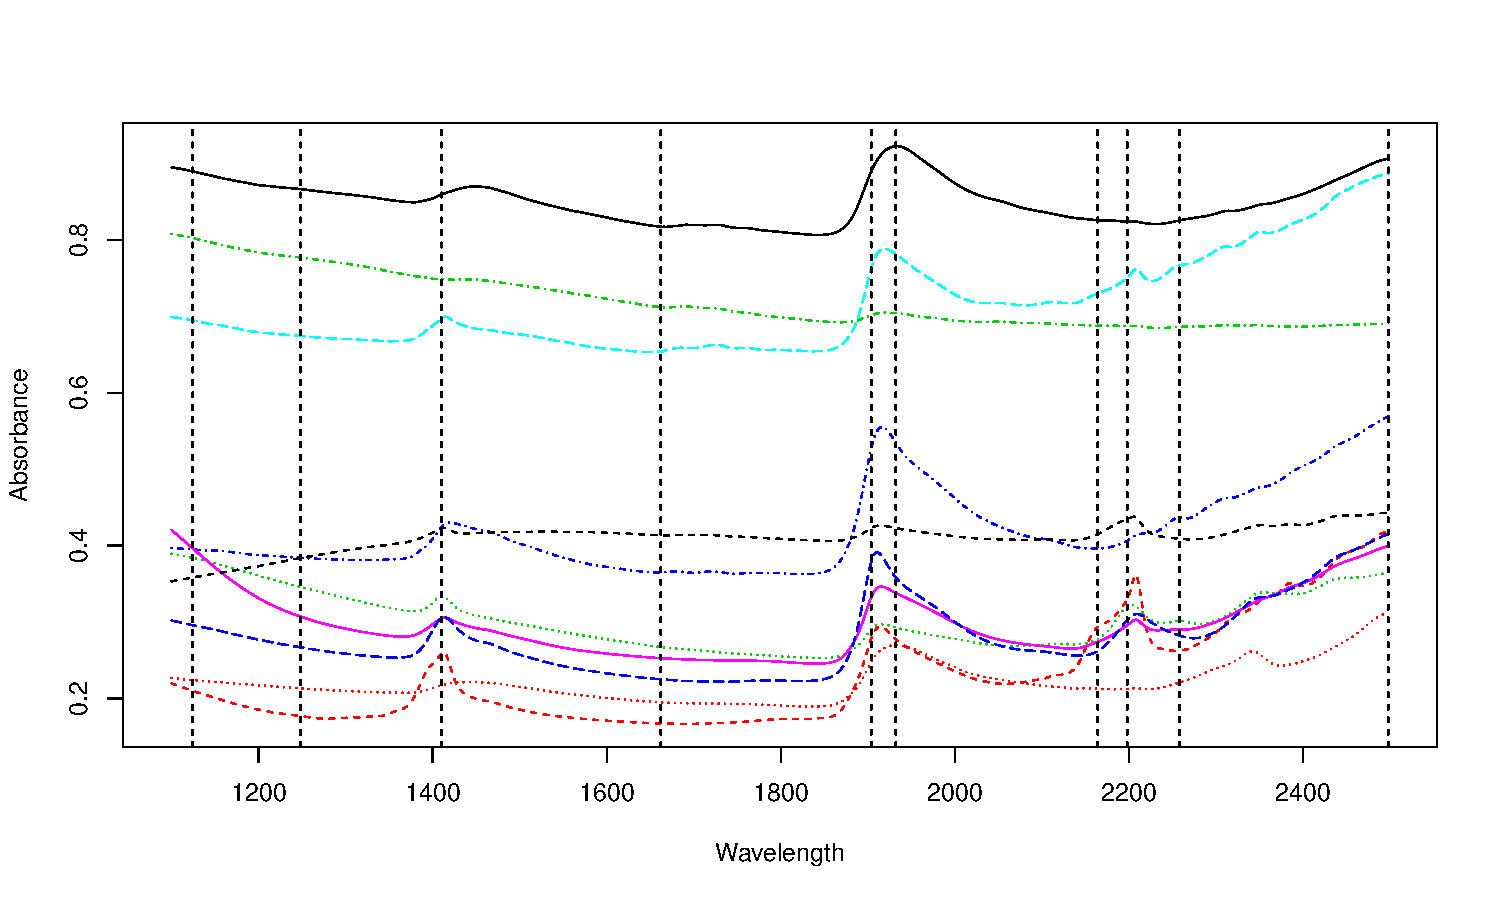
\includegraphics[width=\maxwidth]{figure/honigs} \caption[Spectra selected with the Honigs algorithm and bands used]{Spectra selected with the Honigs algorithm and bands used\label{fig:honigs}}
\end{figure}


\end{knitrout}

  
\bibliographystyle{plain}
\bibliography{prospect-intro}

\end{document}
